\documentclass[a4paper,12pt]{article}

\usepackage[utf8]{inputenc}
\usepackage[T1]{fontenc}
\usepackage[brazil]{babel}
\usepackage{lmodern}
\usepackage{amsmath,amssymb}
\usepackage{graphicx}
\usepackage{booktabs}
\usepackage{array}
\usepackage{geometry}
\usepackage{float}
\usepackage{caption}
\usepackage{hyperref}
\usepackage{xcolor}
\usepackage{listings}
\usepackage{longtable}
\usepackage{microtype}

\geometry{margin=2.5cm}
\hypersetup{colorlinks=true, linkcolor=black, urlcolor=blue, citecolor=black}

\lstdefinestyle{javastyle}{
    language=Java,
    basicstyle=\ttfamily\small,
    keywordstyle=\bfseries,
    commentstyle=\itshape,
    numbers=left,
    numberstyle=\tiny,
    stepnumber=1,
    numbersep=8pt,
    showstringspaces=false,
    breaklines=true,
    frame=single,
    tabsize=4
}
\begin{document}

\begin{titlepage}
    \centering

    \vspace*{3cm}

    {\Large Pontifícia Universidade Católica de Minas Gerais\par}
    \vspace{1cm}

    {\Large Curso de Ciência da Computação\par}
    \vspace{3cm}

    {\LARGE \textbf{Trabalho Prático 01}\\
    Pontes e Caminhos Eulerianos em Grafos\par}

    \vspace{3cm}

    {\large Felipe Tadeu Silva\\
    Mateus Soares Gatti Vasconcellos\par}

    \vfill

    {\large Belo Horizonte\\
    2026}

\end{titlepage}

\begin{abstract}
Este relatório apresenta a implementação e a avaliação experimental de algoritmos para identificação de pontes em grafos simples não direcionados e para obtenção de caminhos e circuitos eulerianos. Foram implementadas duas estratégias para detecção de pontes: uma abordagem ingênua, baseada na remoção individual de arestas e verificação de conectividade, e o algoritmo de Tarjan, baseado em busca em profundidade e valores de menor ancestral alcançável. Além disso, foi implementado o algoritmo de Fleury utilizando cada uma dessas estratégias. Os experimentos foram realizados com grafos eulerianos, semi-eulerianos e não eulerianos contendo 100, 1.000, 10.000 e 100.000 vértices. Os resultados mostram que o método de Tarjan apresenta melhor escalabilidade, enquanto o método ingênuo torna-se inviável em grafos maiores.
\end{abstract}

\section{Introdução}

Grafos são estruturas matemáticas amplamente utilizadas na Ciência da Computação para representar relações entre objetos. Um grafo simples não direcionado pode modelar redes de computadores, rotas, conexões sociais, dependências entre componentes e diversos outros problemas.

Neste trabalho, o foco está em dois conceitos importantes da teoria dos grafos: pontes e caminhos eulerianos. Uma ponte é uma aresta cuja remoção desconecta o grafo. Já um caminho euleriano é um percurso que atravessa todas as arestas exatamente uma vez. A identificação de pontes é particularmente importante no algoritmo de Fleury, pois esse algoritmo evita atravessar pontes quando ainda existem alternativas disponíveis.

O objetivo do trabalho foi implementar duas formas de identificação de pontes, uma ingênua e outra baseada no algoritmo de Tarjan, e comparar seu impacto no algoritmo de Fleury.

\section{Conceitos Teóricos}

\subsection{Pontes}

Seja $G=(V,E)$ um grafo simples não direcionado. Uma aresta $e \in E$ é chamada de ponte se a remoção de $e$ aumenta o número de componentes conexas de $G$. Em outras palavras, uma ponte é uma aresta crítica para manter a conectividade do grafo.

\subsection{Grafos Eulerianos e Semi-Eulerianos}

Um grafo não direcionado possui circuito euleriano quando todos os seus vértices de grau não nulo pertencem à mesma componente conexa e todos possuem grau par. Nesse caso, o percurso começa e termina no mesmo vértice.

Um grafo possui caminho euleriano, mas não circuito, quando exatamente dois vértices possuem grau ímpar. Nesse caso, o caminho começa em um desses vértices ímpares e termina no outro.

Quando o grafo possui quantidade de vértices ímpares diferente de zero ou dois, ele não possui caminho euleriano.

\section{Métodos Implementados}

\subsection{Método Naive para Pontes}

O método Naive testa cada aresta individualmente. Para cada aresta do grafo, a implementação remove temporariamente a aresta e executa uma busca para verificar se o grafo permanece conectado. Se a remoção aumentar o número de componentes conexas, a aresta é classificada como ponte.

A ideia geral do método é:

\begin{enumerate}
    \item Percorrer todas as arestas do grafo.
    \item Remover temporariamente a aresta analisada.
    \item Verificar a conectividade do grafo por busca em profundidade ou largura.
    \item Restaurar a aresta.
    \item Marcar a aresta como ponte caso o grafo tenha ficado desconexo.
\end{enumerate}

A complexidade aproximada desse método é:

\[
O(E \cdot (V+E))
\]

Isso ocorre porque, para cada uma das $E$ arestas, pode ser necessário percorrer vértices e arestas para testar a conectividade.

\subsection{Algoritmo de Tarjan para Pontes}

O algoritmo de Tarjan identifica pontes usando uma única busca em profundidade. Durante a DFS, são armazenados dois valores principais:

\begin{itemize}
    \item $disc[u]$: tempo de descoberta do vértice $u$.
    \item $low[u]$: menor tempo de descoberta alcançável a partir de $u$, considerando arestas de árvore e arestas de retorno.
\end{itemize}

Durante a DFS, uma aresta $(u,v)$ é ponte quando:

\[
low[v] > disc[u]
\]

Essa condição significa que o vértice $v$ e sua subárvore não conseguem alcançar nenhum ancestral de $u$ sem utilizar a aresta $(u,v)$. Logo, a remoção dessa aresta desconectaria o grafo.

A complexidade desse método é:

\[
O(V+E)
\]

Portanto, Tarjan é muito mais adequado para grafos grandes.

\subsection{Algoritmo de Fleury}

O algoritmo de Fleury constrói um caminho ou circuito euleriano removendo as arestas percorridas. Em cada passo, ele escolhe uma aresta que não seja ponte, sempre que houver mais de uma opção disponível. Caso a única opção restante seja uma ponte, ela pode ser utilizada.

A implementação foi executada de duas formas:

\begin{itemize}
    \item Fleury com identificação de pontes pelo método Naive.
    \item Fleury com identificação de pontes pelo algoritmo de Tarjan.
\end{itemize}

Antes de tentar construir o percurso, a implementação classifica o grafo como euleriano, semi-euleriano ou não euleriano. Para grafos não eulerianos, o algoritmo informa que não existe caminho euleriano.

\section{Metodologia Experimental}

Foram utilizados grafos aleatórios com os seguintes tamanhos:

\begin{itemize}
    \item 100 vértices;
    \item 1.000 vértices;
    \item 10.000 vértices;
    \item 100.000 vértices.
\end{itemize}

Para cada tamanho, foram gerados três tipos de grafos:

\begin{itemize}
    \item Euleriano;
    \item Semi-euleriano;
    \item Não euleriano.
\end{itemize}

A medição de tempo foi feita em milissegundos usando média de múltiplas execuções. Para evitar execuções excessivamente longas, alguns casos foram marcados como \textit{N/A (lento)} ou \textit{N/A (impraticável)}. Isso ocorreu principalmente no método Naive em grafos maiores e no algoritmo de Fleury para grafos com 100.000 vértices.

\section{Resultados Funcionais}

A primeira validação consistiu em executar os algoritmos em grafos pequenos, com 100 vértices, para verificar se os dois métodos de identificação de pontes produziam resultados equivalentes. A implementação indicou concordância entre o método Naive e o método de Tarjan nos grafos testados.

Nos grafos eulerianos, foi encontrado circuito euleriano. Nos grafos semi-eulerianos, foi encontrado caminho euleriano. Nos grafos não eulerianos, o algoritmo corretamente indicou que não existe caminho euleriano.

\section{Resultados dos Experimentos}

\subsection{Experimento 1: Identificação de Pontes}

A Tabela \ref{tab:pontes} apresenta os tempos médios obtidos para identificação de pontes. Os valores estão em milissegundos.

\begin{table}[H]
\centering
\caption{Tempo médio para identificação de pontes.}
\label{tab:pontes}
\begin{tabular}{llrrr}
\toprule
Tipo & Vértices & Arestas & Naive (ms) & Tarjan (ms) \\
\midrule
Euleriano & 100 & 108 & 0.796 & 0.011 \\
Semi-euleriano & 100 & 111 & 0.466 & 0.007 \\
Não euleriano & 100 & 124 & 0.264 & 0.012 \\
Euleriano & 1.000 & 1.017 & 22.030 & 0.074 \\
Semi-euleriano & 1.000 & 1.025 & 19.576 & 0.096 \\
Não euleriano & 1.000 & 1.249 & 36.695 & 0.056 \\
Euleriano & 10.000 & 10.017 & N/A & 0.552 \\
Semi-euleriano & 10.000 & 10.014 & N/A & 0.523 \\
Não euleriano & 10.000 & 12.497 & N/A & 1.267 \\
Euleriano & 100.000 & 100.019 & N/A & 8.469 \\
Semi-euleriano & 100.000 & 100.017 & N/A & 8.167 \\
Não euleriano & 100.000 & 124.999 & N/A & 18.520 \\
\bottomrule
\end{tabular}
\end{table}

\begin{figure}[H]
\centering
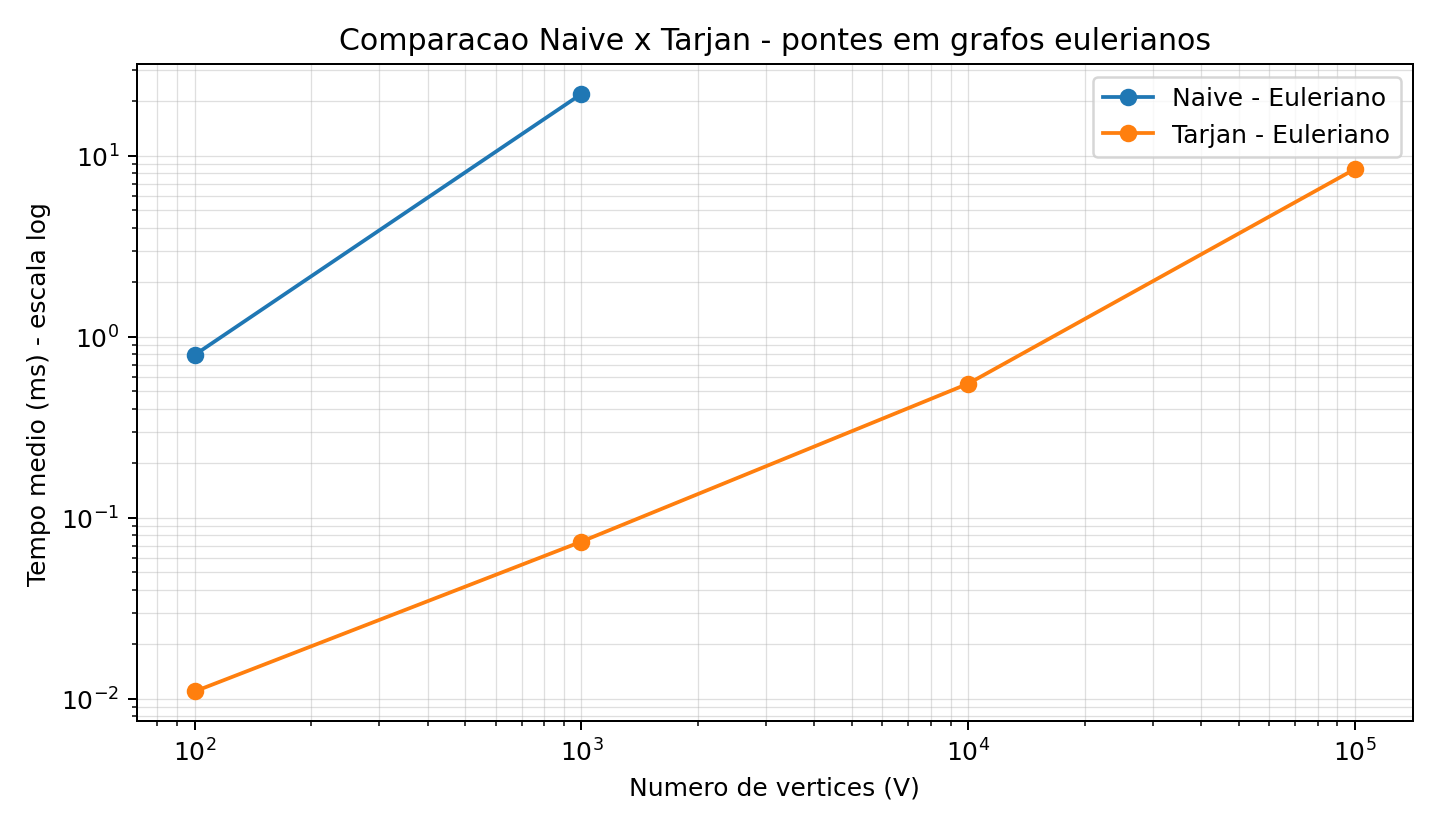
\includegraphics[width=0.92\textwidth]{grafico_comparacao_pontes.png}
\begin{figure}
    \centering
    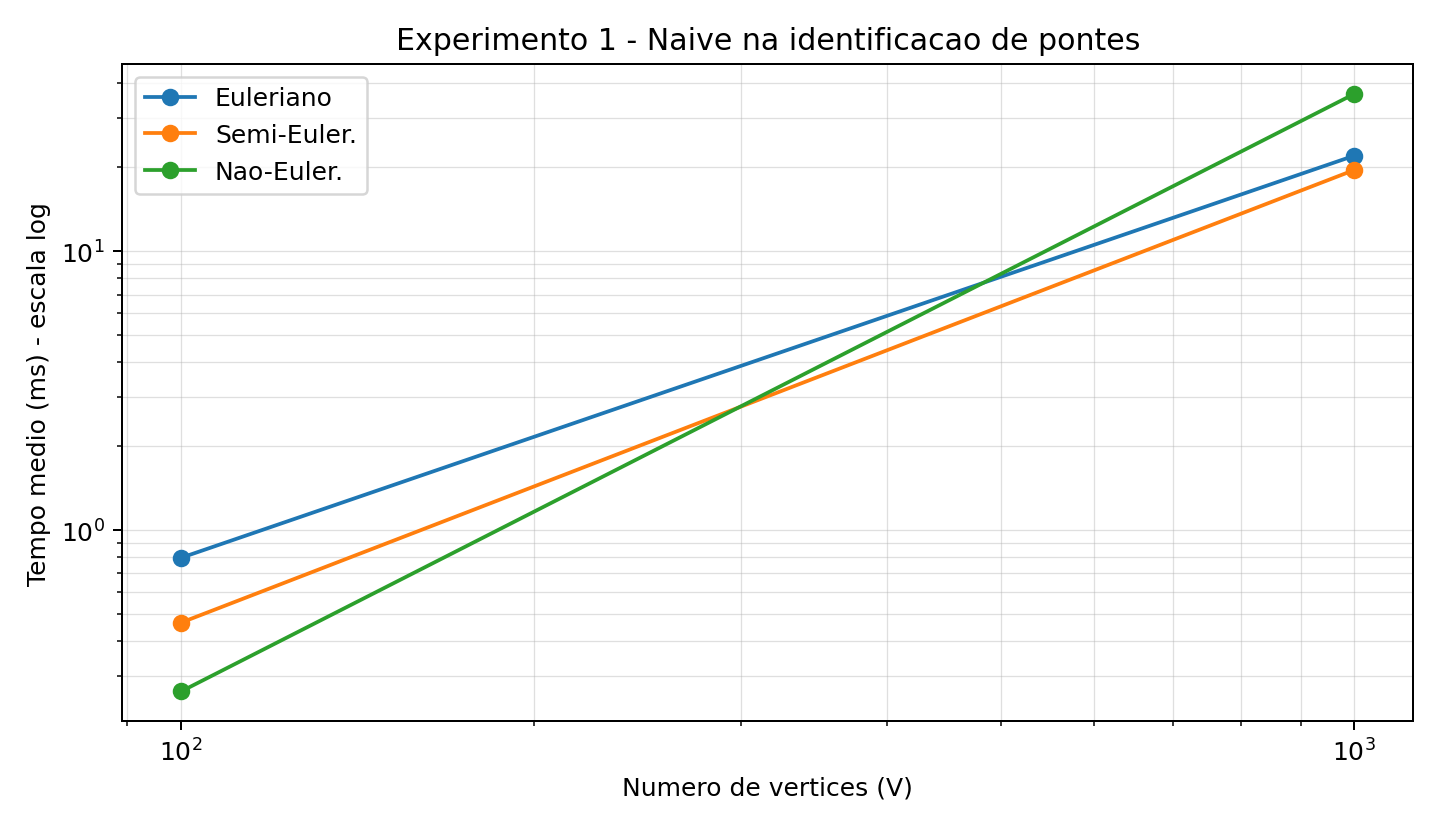
\includegraphics[width=0.92\linewidth]{grafico_naive_pontes.png}
    \caption{Enter Caption}
    \label{fig:placeholder}
\end{figure}
\caption{Comparação entre Naive e Tarjan para identificação de pontes em grafos eulerianos.}
\label{fig:comparacao-pontes}
\end{figure}

\begin{figure}[H]
\centering
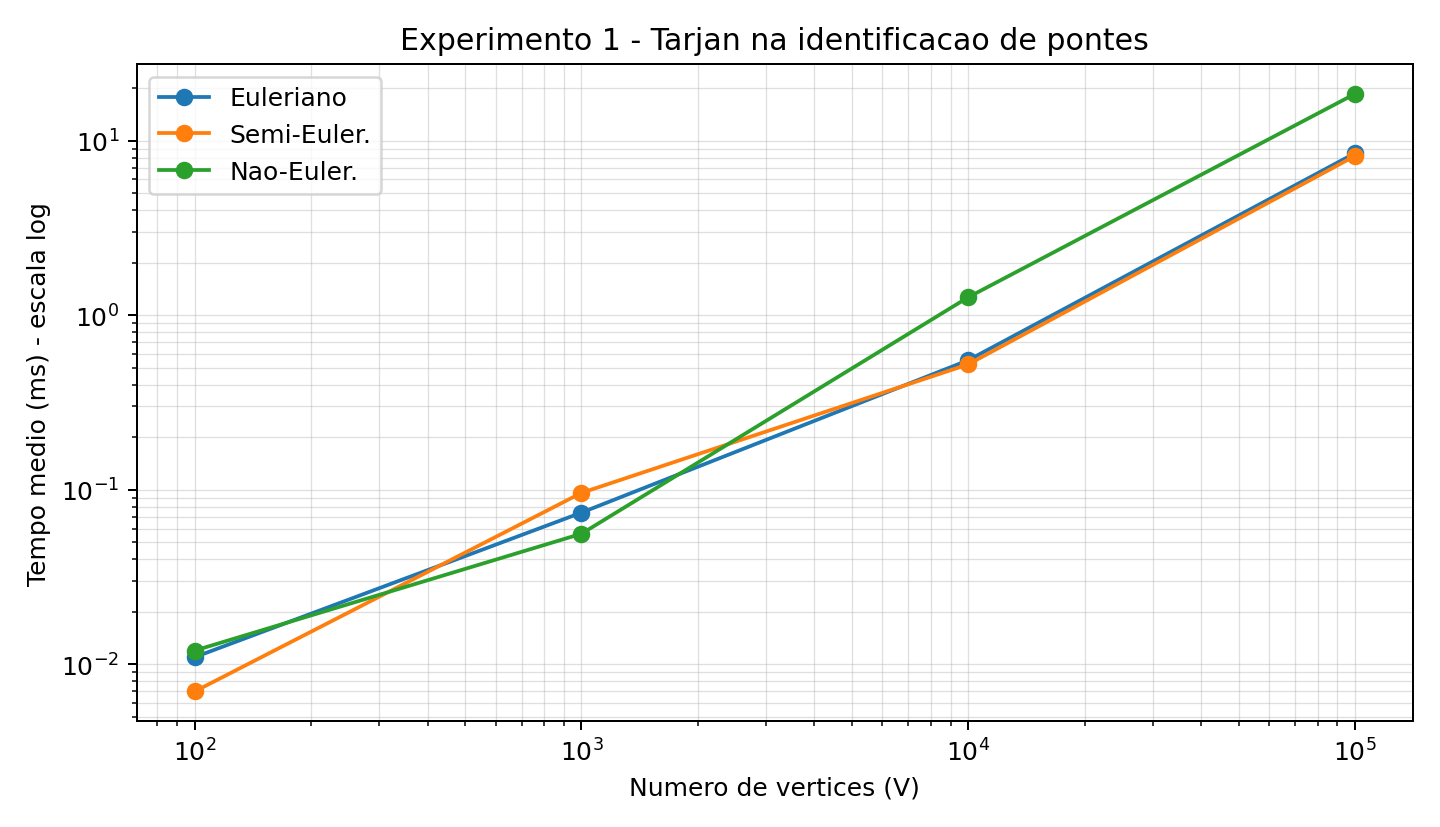
\includegraphics[width=0.92\textwidth]{grafico_tarjan_pontes.png}
\caption{Crescimento do tempo do algoritmo de Tarjan na identificação de pontes.}
\label{fig:tarjan-pontes}
\end{figure}

\begin{figure}[H]
\centering
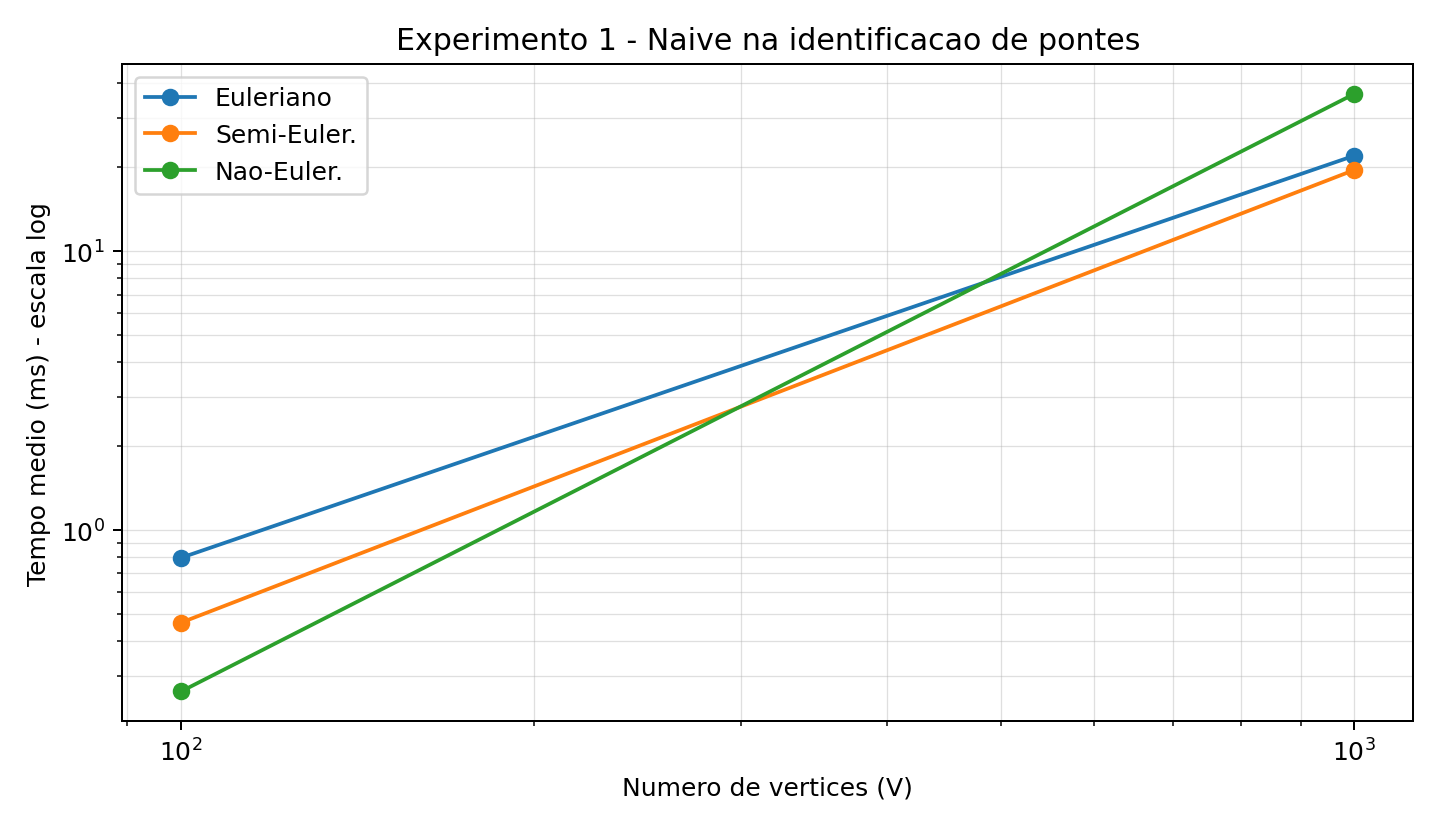
\includegraphics[width=0.92\textwidth]{grafico_naive_pontes.png}
\caption{Crescimento do tempo do método Naive na identificação de pontes.}
\label{fig:naive-pontes}
\end{figure}

\subsection{Experimento 2: Algoritmo de Fleury}

A Tabela \ref{tab:fleury} apresenta os tempos médios do algoritmo de Fleury. Para grafos não eulerianos, o algoritmo não executa o percurso completo, pois não existe caminho euleriano.

\begin{table}[H]
\centering
\caption{Tempo médio do algoritmo de Fleury.}
\label{tab:fleury}
\begin{tabular}{llrrr}
\toprule
Tipo & Vértices & Arestas & Naive (ms) & Tarjan (ms) \\
\midrule
Euleriano & 100 & 109 & 5.713 & 0.261 \\
Semi-euleriano & 100 & 110 & 5.562 & 0.264 \\
Não euleriano & 100 & 124 & N/A & N/A \\
Euleriano & 1.000 & 1.017 & N/A & 18.360 \\
Semi-euleriano & 1.000 & 1.017 & N/A & 19.695 \\
Não euleriano & 1.000 & 1.249 & N/A & N/A \\
Euleriano & 10.000 & 10.016 & N/A & 3217.544 \\
Semi-euleriano & 10.000 & 10.023 & N/A & 3332.781 \\
Não euleriano & 10.000 & 12.498 & N/A & N/A \\
Euleriano & 100.000 & 100.028 & N/A & N/A \\
Semi-euleriano & 100.000 & 100.024 & N/A & N/A \\
Não euleriano & 100.000 & 124.999 & N/A & N/A \\
\bottomrule
\end{tabular}
\end{table}

\begin{figure}[H]
\centering
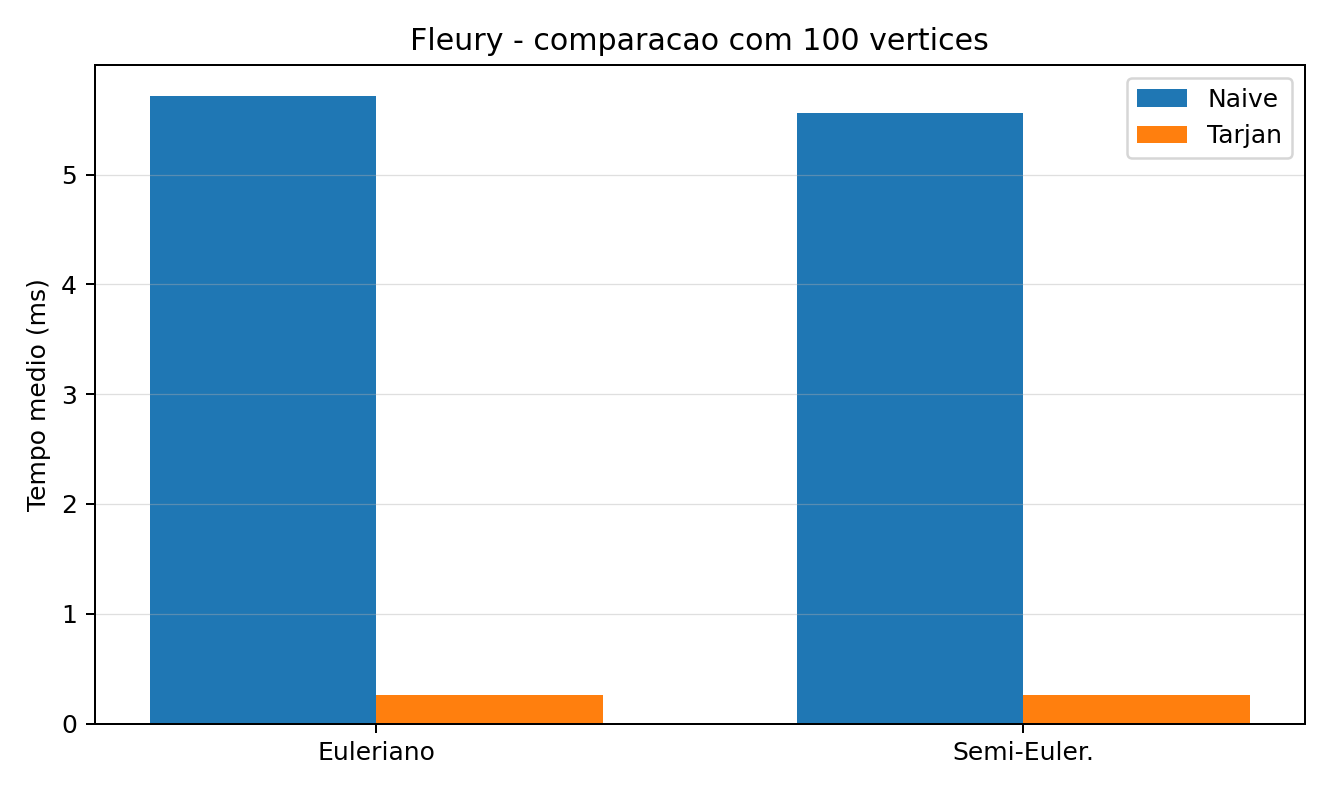
\includegraphics[width=0.92\textwidth]{grafico_fleury_100.png}
\caption{Comparação entre Fleury com Naive e Fleury com Tarjan para 100 vértices.}
\label{fig:fleury-100}
\end{figure}

\begin{figure}[H]
\centering
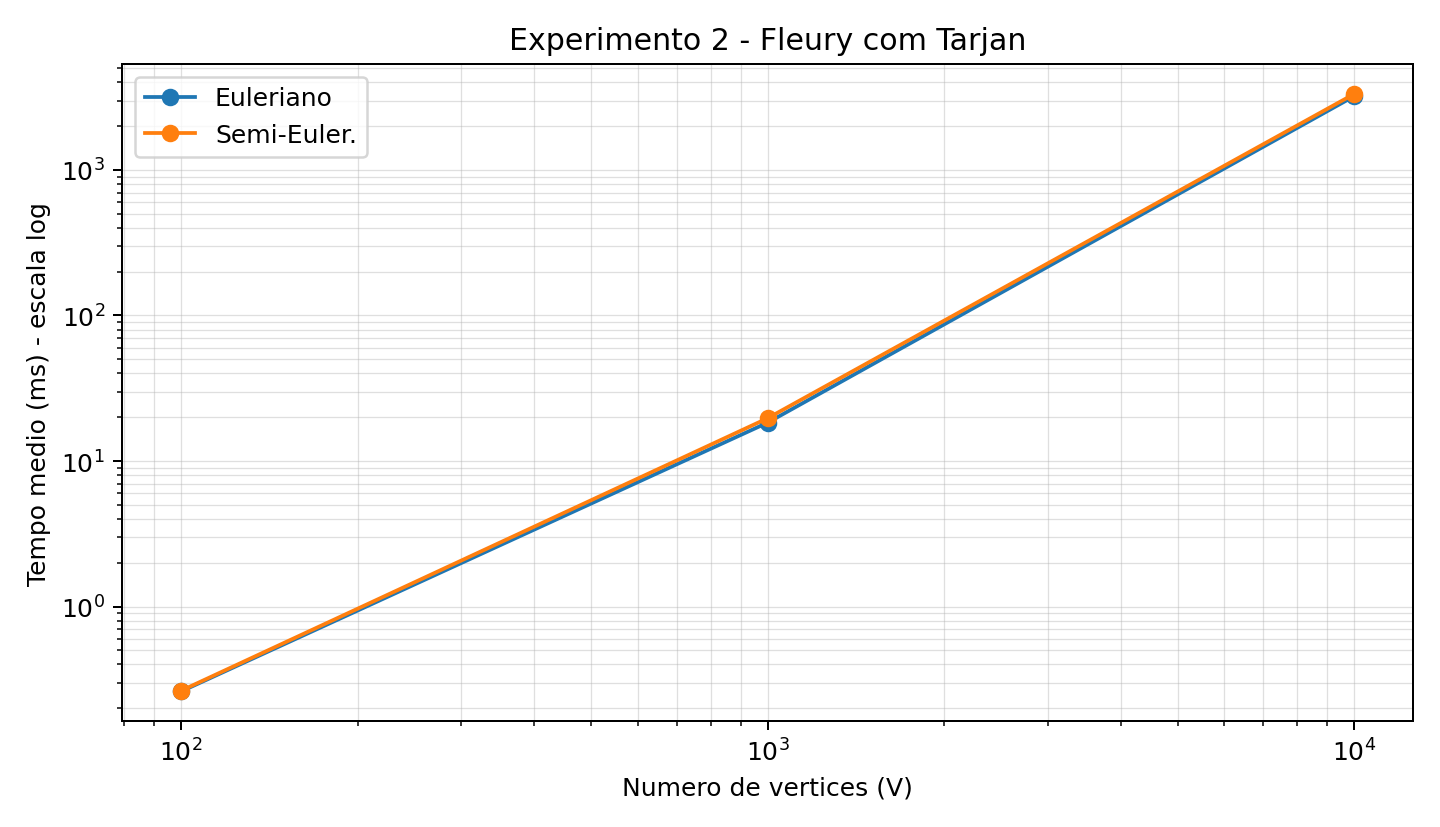
\includegraphics[width=0.92\textwidth]{grafico_fleury_tarjan.png}
\caption{Crescimento do tempo do algoritmo de Fleury utilizando Tarjan.}
\label{fig:fleury-tarjan}
\end{figure}

\section{Análise dos Resultados}

Os resultados do primeiro experimento mostram uma diferença significativa entre os dois métodos de identificação de pontes. Para grafos com 100 vértices, ambos os métodos executam rapidamente. Entretanto, quando o tamanho aumenta para 1.000 vértices, o método Naive já apresenta tempos dezenas ou centenas de vezes maiores que Tarjan.

Nos grafos com 10.000 e 100.000 vértices, o método Naive foi considerado inviável dentro do limite de tempo adotado. Isso confirma sua limitação prática, causada pela necessidade de testar a conectividade do grafo após a remoção de cada aresta.

O algoritmo de Tarjan apresentou crescimento muito mais controlado. Mesmo em grafos com 100.000 vértices, os tempos permaneceram baixos, variando de aproximadamente 8 ms a 18 ms nos testes realizados. Esse comportamento está de acordo com sua complexidade linear $O(V+E)$.

No segundo experimento, observa-se que o algoritmo de Fleury é mais custoso do que a simples identificação de pontes. Isso ocorre porque, durante a construção do caminho euleriano, o algoritmo precisa decidir repetidamente se uma aresta deve ou não ser utilizada. Com o método Naive, essa decisão se torna muito cara, tornando o algoritmo inviável já a partir de grafos com 1.000 vértices. Com Tarjan, o algoritmo conseguiu executar até 10.000 vértices, mas passou a apresentar tempos na ordem de segundos.

Portanto, embora Tarjan seja muito eficiente para identificar todas as pontes de um grafo, o algoritmo de Fleury ainda possui limitações para grafos muito grandes, pois realiza decisões sucessivas durante o percurso euleriano.

\section{Conclusão}

O trabalho permitiu comparar duas estratégias para identificação de pontes em grafos e analisar seu impacto no algoritmo de Fleury. O método Naive é simples e fácil de implementar, mas apresenta desempenho inadequado para grafos grandes. Já o algoritmo de Tarjan é muito mais eficiente, pois identifica pontes em tempo linear.

Os experimentos confirmaram a superioridade de Tarjan na identificação de pontes. Além disso, mostraram que o algoritmo de Fleury depende fortemente do método usado para detectar pontes. A versão com Naive torna-se impraticável rapidamente, enquanto a versão com Tarjan apresenta desempenho melhor, embora ainda limitado para grafos muito grandes.

Assim, conclui-se que a escolha do algoritmo de identificação de pontes é essencial para a eficiência da solução. Para aplicações práticas envolvendo grafos grandes, o método de Tarjan é a alternativa mais adequada entre as duas estratégias analisadas.

\section{Referência}

Tarjan, R. E. (1974). \textit{A note on finding the bridges of a graph}. Information Processing Letters, 2(6), 160-161. \url{https://doi.org/10.1016/0020-0190(74)90003-9}


\end{document}
